\begin{figure*}[t]
\centering
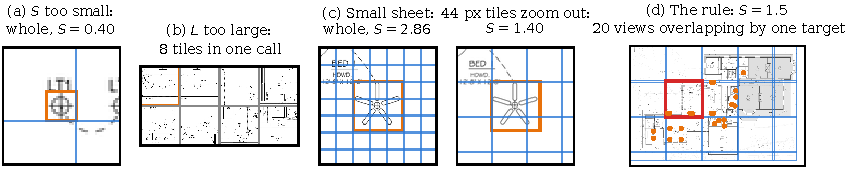
\includegraphics[width=\textwidth]{figures/fig1.pdf}
\caption{The two quantities and the fix. $S$ is how many visual tokens an object spans per side; $L$ is how much one call must search and report. (a) An $\CfigW{} \times \CfigH$ px sheet sent whole within 2{,}500 tokens of 32 px: one of its \CfigTargets{} targets spans $S = \CfigSwhole$ tokens (blue: token grid; orange: target box). (b) Packing eight same-scale tiles into one call keeps $S$ and raises $L$; for GPT-5.6, recall on the 14 full sheets falls from \XmosRgptFiveSixkOne{} to \XmosRgptFiveSixkEight, although a packed call must report a median of only \CpackMedian{} targets. (c) A pixel-defined recipe (44 px symbols, 1{,}024 px tiles) zooms in on large sheets but out on a small one, from $S = \CsmallSw$ to \CsmallSt; GPT-5.4's recall falls from \CsmallRecWhole{} to \CsmallRecTile. (d) The rule of \cref{sec:safe}: \CfigViews{} views at $S = 1.5$ that overlap by one target, \CfigTokens{} tokens in total, against the minimum of \cref{thm:exact}(c) for any split that protects the sheet at this $S$ (blue: view borders; red: one view; orange dots: targets). (a), (c), (d): 32 px tokens, 2{,}500 per image; (a) and (c) show the pixels the model receives. Recalls in (b) and (c) are measured.}
\label{fig:intro}
\end{figure*}

\section{Introduction}
\label{sec:intro}

Many images people work with are large and dense: a high-resolution screenshot holds dozens of icons and controls, a document page hundreds of fields and marks, an engineering drawing hundreds of symbols, and there are shelf photographs, maps, tissue slides and satellite scenes. The objects are small and many, and their kinds change from task to task, so training a detector for each rarely pays. Vision-language models (VLMs) turn this into one instruction and one example, and they are becoming the perception layer of computer-use, document and design agents~\cite{su2025thinkingwithimages,zheng2026deepeyes}. But a VLM sees an image through a fixed token budget and misses small objects. Every user, and every agent that calls a VLM, must decide whether to send the image whole, raise its resolution, split it, or zoom, and the choices differ several-fold in accuracy and cost.

\paragraph{Our answer, in brief.}
VLMs miss small objects for two reasons that a caller can estimate before any call: an object gets too few visual tokens, and a call must search and report too much. Splitting the image cannot lower expected recall when no view zooms out and views overlap by one object, and neither part of this condition can be dropped. The guarantee assumes the model is monotone, which held on every standard input we tested (\cref{sec:safe}) and failed only when OpenAI models were sent larger images than our standard input (images we resize ourselves so that the vendor need not, \cref{sec:protocol}). In short: \emph{never zoom out, and overlap views by one object}. Protecting every target at a given $S$ has a minimum token price that no split avoids, and a simple rule pays it up to an explicit factor, so a caller can decide before any call how to send an image and what it will cost, for future models too. On the newest models, the rule raises recall most where the whole image gives targets the fewest tokens (\cref{sec:practice}).

\paragraph{Two quantities and their price.}
Each call gives the model an image and an example of the target and asks for the centre of every instance; a point counts if it lies within half a target of an instance not already matched. $S$ says whether the model can see the target (the object to find): the target's side in the image the model receives, in units of one visual token ($S = 1.5$: one and a half tokens wide). It follows from public interface rules and the image size, with no label and no call. An $\CfigW{} \times \CfigH$ px drawing sent whole within 2{,}500 tokens of 32 px shrinks its \CfigM{} px symbols to about \CfigMsent{} px, \CfigPctToken\% of a token ($S = \CfigSwhole$, \cref{fig:intro}a). $L$ says how much one call must do: \emph{search} a view, with its targets, look-alikes and lines, and \emph{report} one accurate position per target. If $S$ is the size of the print, $L$ is how many pages one must proofread at once; clear print does not help when too many pages arrive together.
The two fixes are priced very differently. Seeing a whole image at $S$ takes at least its area over the target's area times $S^2$ tokens, and more with the margins that protect every target, so raising $S$ by a factor $a$ raises this minimum $a^2$-fold: the drawing above needs at least about \CfigCmin{} tokens at $S = 1.5$, against 2{,}500 sent whole. Splitting into $k$ views at the same scale cuts each view's area to about $1/k$ at a cost at most linear in $k$: nearly free for models billed by resolution (GPT, Claude, Qwen), and $k$ images for fixed-grid models (Gemini), which also raises their $S$. A high-resolution mode raises $S$ but keeps $L$ at the whole image; a zoom agent sets both region by region.

\paragraph{Three surprises that the two quantities explain.}
\emph{More pixels can hurt}: sent through GPT-5.6's high-resolution mode with reasoning, the 14 full drawing sheets give each target more tokens, yet F1 falls from \XnFAOneRgptFiveSixSheets{} at 1{,}600 px to \XnFNATRgptFiveSixSheets; on this input path (the route by which an image reaches the model) the model stops satisfying ``more tokens do not hurt''. \emph{Splitting can zoom out}: recipes that rescale an image to a pixel size before tiling ignore how the vendor rescales the whole image. A 44 px recipe (44 px symbols, 1{,}024 px tiles) raises $S$ on the large drawing from \CfigSwhole{} to about 1.4 but lowers it on a $\CsmallW{} \times \CsmallH$ px drawing from \CsmallSw{} to \CsmallSt, and on this sheet GPT-5.4's recall falls from \CsmallRecWhole{} to \CsmallRecTile{} (\cref{fig:intro}c); where symbols were already large, it lowered recall in \XtcOutNegPoint{} of \XtcOutN{} model and data settings, significantly in \XtcOutNeg. \emph{Seeing has a price}: the bound above holds for every split that sees the whole image at $S$, whoever splits. Such effects are found by trial, and answers tuned for one model expire with the next; theorems can give what trial cannot: conditions checked before a call, guarantees for every model with two testable properties, a cost no protected split can beat, and conditions whose parts are each necessary, which explains both failures. We test them in about \CscaleCalls{} requests to \CscaleModels{} models, including the newest generation, on \CscaleImages{} images with about \CscaleInst{} instances.

\begin{answerbox}
\textbf{Three answers.}
\textbf{(1) Why VLMs miss small objects:} too few tokens per object ($S$) and too much to search and report in one call ($L$). The interface caps $S$ and prices seeing, the same for every model (\cref{sec:why}).
\textbf{(2) What better models change:} they need less $S$ and handle more per call, so fewer images need splitting. But an image can be arbitrarily large while a call's budget is fixed, so seeing a whole image keeps a minimum cost, for zoom agents too, and splitting does not become obsolete (\cref{sec:why}).
\textbf{(3) When splitting is safe and what it costs:} no zoom-out and one object of overlap, with monotonicity, suffice, and neither part can be dropped; protection has a minimum cost and a rule pays it up to an explicit factor; the guarantee degrades gracefully. What changes is who splits: the caller, a zoom tool or the model (\cref{sec:safe,sec:practice}).
\end{answerbox}

\begin{table}[t]
\centering
\small
\setlength{\tabcolsep}{2pt}
\begin{adjustbox}{max width=\linewidth}\begin{tabular}{lccc}
\toprule
Model & Budget $N$ & Targets & Targets \\
 & per view & per side & per call \\
\midrule
GPT-6.1 (GPT-5.6) & 8{,}192 & about \CthumbSideGpt{} & 300+ (about 130) \\
Claude Opus 5.5 & 4{,}784 & about \CthumbSideClaude{} & about 130 \\
Gemini 4 (Gemini 3.8) & about 1{,}090 & about \CthumbSideGemini{} & 40+ (about 16) \\
Qwen3-VL & about 2{,}500 & about \CthumbSideQwen{} & about 16 \\
\bottomrule
\end{tabular}\end{adjustbox}
\caption{A rule of thumb at $S = 1.5$: values at pooled recall about 0.9 on 12 controlled images per target count, for one image content (one target type among three look-alike types), with the reasoning settings of \cref{sec:protocol}; in parentheses, the previous model of the vendor; ``+'': a full view showed no drop. Budget $N$ in tokens; targets per side: about $\sqrt{N}/1.5$. Details in \supp{L}.}
\label{tab:thumb}
\end{table}

\paragraph{What a user can take away.}
The rule protects at $S^\ast = 1.5$, above every model's half-recall point (\cref{sec:why}); the $L$ a call can carry grows with each generation (\cref{tab:thumb}). A rule of thumb needs only the target's size $m$ in pixels, the image size and the per-view budget $N$:
\textbf{(i) If the target is small, enlarge} it to about 48 px in the sent image (GPT, Qwen; 32 px tokens) or 42 px (Claude; 28 px tokens); fixed-grid models skip this step.
\textbf{(ii) If the image is large, split} it into views without zooming out. Use $S = \max(1.5, \Sw)$, where $\Sw$ is the $S$ of the whole image; each view is then at most about $m\sqrt{N}/S$ pixels, or $\sqrt{N}/S$ targets, on a side, and overlaps its neighbours by one target.
\textbf{(iii) If targets are many or the content busy, split further} at the same scale, to about the counts in \cref{tab:thumb}.
In all our data, splits that never zoom out raised recall by \CmapBelowMin{} to \CmapBelowMax{} on average where $S < 1.5$, and splits that zoom out lowered it by \CmapZoomMin{} to \CmapZoomMax{} (\cref{fig:map}).

\paragraph{Contributions.}
\textbf{(1) When splitting is safe and how little it can cost, answered exactly and constructively.} ``No zoom-out, one object of overlap'' guarantees that splitting does not lower expected recall for every monotone model, and each part is necessary. Every protected split pays a minimum token cost, and a directly executable rule pays at most this minimum times an explicit factor that tends to one for ideal views; with approximate assumptions, recall degrades by at most the measured defects. The condition covers every local task with one position and one answer per object, including detection and segmentation.
\textbf{(2) Why VLMs miss small objects, in one interface-level account that also predicts future models.} The interface caps $S$ and prices seeing, quadratically for $S$ and at most linearly for $L$; models set the $S$ they need and what one call can handle; a frontier of the same $S^2$ form binds every search strategy, zoom agents included, whenever recognition is graded, so better models do not make splitting obsolete; \cref{sec:future} says where the next models should improve.
\textbf{(3) Tests at scale, including the newest models.} Across \CscaleModels{} models, controlled tests give the assumptions measurable content; across all data, splits that never zoom out gain where $S$ is low and splits that zoom out lose; in \CtCells{} model and data settings the rule raised recall significantly in \CtSigRec{} and precision and F1 in \CtSigPrec, most where the whole image gives targets the fewest tokens, at a cost computable in advance; the effects of $S$ and $L$ carry over to natural images and zoom agents.
We release the LegendSpot benchmark (40 architectural drawings, 1{,}028 instances of legend symbols), a planning tool for safe splitting, the code and all model outputs at \url{https://github.com/shijunzhe/vlm-small-objects} (\supp{K}).
